%*********************************************************************
%TJGDthesis:天津工业大学本科生毕业论文Latex排版示例 非官方
%Copyright 2021 Liwei-522Moeyu  
%2021/04/20 v1.3.1 beta  
%
%**重要提示:**  
%		1. LaTex模板参考2020 Qiu Renxiang-中国人民大学本科生毕业论文模板 
%		2. 提供可单独使用的docx模板,docx模板与文件夹bib、image不产生关联
%		3. LaTex模板请确保使用 UTF-8 编码保存  
%		4. LaTex模板请使用 XeLaTeX编译  
%		5. LaTex模板修改、使用、发布本文档请务必遵循 LaTeX Project Public License  
%		6. 请删除不必要的注释  
%		7. LaTex模板请切换默认文献工具为biber  
%		8. 参与修订请联系:moeyu522@qq.com 或参与GitHub Issues
%		9. 文件结构:  
%		    TJGDthesis  
%		---- doc[相关规定说明文件] 
%		---- bib[文献存放,内含后缀为.bib文件]  
%		---- image[图片存放]  
%		---- TJGDthesis.docx[可单独使用]  
%		-----TJGDthesis.tex  
%蓝奏云链接:  
%https://wwe.lanzous.com/b010ayxaj
%地址访问密码: TJGD
%压缩包解压密码:TJGD  
%
%不再提供Gitee仓库链接
%
%本项目GitHub地址:
%https://github.com/moeyu522/TJGDthesis
%
%**致谢**  
%感谢室友波提出的整改意见,感谢室友豪,室友毛在本人完成模板期间的带饭,阿里嘎多。
%
%**update log**  
%- 2021/6/5 v1.3.1 将名称改为Latex排版示例,添加相关的官方说明,其中2018版为计算机学院广泛采用的排版,修改页边距,添加附录章节,封面增加学号,除封面外,其他部分与2018版本不一致
%- 2021/04/20 v1.3  删除latex模板中摘要页页脚,docx文档版本与latex模板同一为v1.3,docx模板修改些许细节问题  
%- 2021/03/18  v1.2  添加docx文档  
%- v1.1  初始化tex文档 
%*********************************************************************
\documentclass[a4paper,zihao=-4,UTF8]{ctexart}
%所需的包
\usepackage{geometry}
\usepackage[T1]{fontenc}
%Times New Roman字体
\usepackage{mathptmx}
\usepackage{hyperref}
\usepackage{fancyhdr}
\usepackage{fontspec}
\usepackage{xeCJK}
\usepackage{ulem}
\usepackage{xfakebold}
\usepackage{titlesec}
\usepackage{graphicx}
\usepackage{booktabs}
\usepackage[style=gb7714-2015]{biblatex}
\usepackage{amsmath}
\usepackage{chngcntr}
\usepackage{caption}
\usepackage{titletoc}
\usepackage{zhnumber}
%设置图片表格的标题为10.5pt
\captionsetup{font={small}}
%公式,图片表格编号跟随章节
\numberwithin{equation}{section}
\counterwithin{figure}{section}
\counterwithin{table}{section}
%使用\bold{}来加粗中文字体
\newcommand{\bold}[2][0.3]{\setBold[#1]#2\unsetBold}

%设置英文正文字体
\setmainfont{Times New Roman}
%设置中文正文字体-宋体
\setCJKmainfont{SimSun}

%全文默认行间距Word版本的1.25倍
\linespread{1.04}

\geometry{a4paper,left = 3.18cm,right = 3.18cm,top = 2.54cm,bottom= 2.54cm}

%目录和引用超链接
\hypersetup{
	colorlinks=true,
	linkcolor=black,
	citecolor=black
}

%页眉
\pagestyle{fancy}

%引用参考文献
\addbibresource{./bib/references.bib}

%正文开始
\begin{document}
	
%封面
\begin{titlepage}
	\vspace*{24mm}
	\centering 
	
	\zihao{1}{\heiti\bold{天津工业大学}}
	
	\vspace{3mm}
	
	\zihao{2}{\songti{本科生毕业设计(论文)}}
	
	\vspace{12mm}
	\zihao{3} \bold{题目:}{论文的题目}
	
	\vspace{60mm}
	
	\zihao{3}{\bold{学\qquad 号:\uline{\makebox[78mm][c]{5201314}}}}
	
	\zihao{3}{\bold{姓\qquad 名:\uline{\makebox[78mm][c]{李伟}}}}
	
	\zihao{3}{\bold{专\qquad 业:\uline{\makebox[78mm][c]{xxxxx}}}}
	
	\zihao{3}{\bold{学\qquad 院:\uline{\makebox[78mm][c]{计算机科学与软件学院}}}}
	
	\zihao{3}{\bold{指导教师:\uline{\makebox[78mm][c]{xxxxx}}}}
	
	\zihao{3}{\bold{职\qquad 称:\uline{\makebox[78mm][c]{xxxx}}}}
	
	\zihao{3}{\bold{完成日期:\uline{\makebox[78mm][c]{xxx年xxx月xxx日}}}}
	
\end{titlepage}

\newpage

%关闭页眉
\fancyhf{}
\renewcommand{\headrulewidth}{0pt}
%中文摘要环境
\renewcommand{\abstractname}{\zihao{3}\heiti 摘\qquad 要}
\renewenvironment{abstract}{
	\par\zihao{-4}
	\noindent\mbox{}\hfill{\abstractname}\hfill\mbox{}\par
	\vskip 2.5ex}{\par\vskip 2.5ex}
\begin{abstract}
	近年来互联网的广泛使用引发了信息的爆炸式增长,个性化推荐系统作为解决“信息过载”问题的有效工具应运而生,通过算法帮助用户过滤信息,减少了用户需要处理的信息量。目前,个性化推荐系统已经广泛应用于搜索引擎、电子商务、社交娱乐等网络平台,在人们日常使用的过程中随处可见。然而,个性化推荐系统的广泛应用也带来了“信息窄化”、用户信息泄露等问题,个性化推荐系统对于用户信息搜寻成本的具体影响变得更为复杂。
	
	本文将用结构方程模型来分析信息搜寻成本的变化对个性化推荐系统的用户使用意愿的影响情况。
	
	基于研究得出的结论,本文从现实中存在的个性化推荐精度不足、信息窄化以及个人信息的侵害等方面的问题出发,提出了对于未来个性化推荐优化的展望。在算法方面,通过使用深度学习与知识图谱等前沿技术与算法提高个性化推荐的精确程度。在个人信息使用与信息窄化的问题上,平台可以增加相应调节选项,提高用户的自主选择性。其次,也可以通过提高推荐过程的可解释性来增强用户对推荐系统的信任度与满意度。另外,还需要政府部门完善个人信息保护的法律法规、社会舆论与公共部门发挥监督与监管作用,以及企业上下游齐发力,共同降低个人隐私泄露的风险。
	
	\vspace{12mm}
	\raggedright
	\zihao{-4}{\heiti\bold{关键词:}}
	\zihao{-4}{\songti{关键词1; 关键词2;关键词3;关键词4}}
\end{abstract}
%v1.3add 版本删除中文英文摘要的页脚
%罗马字编码
%\setcounter{page}{1}
%\pagenumbering{Roman}
%\cfoot{\footnotesize \thepage}

\newpage

%英文摘要环境
\newcommand{\enabstractname}{\textbf{\zihao{3} Abstract}}
\newenvironment{enabstract}{
	\par\zihao{-4}
	\noindent\mbox{}\hfill{\enabstractname}\hfill\mbox{}\par
	\vskip 2.5ex}{\par\vskip 2.5ex}
\begin{enabstract}
	There are moments in life when you miss someone so much that you just want to pick them from your dreams and hug them for real! Dream what you want to dream;go where you want to go;be what you want to be,because you have only one life and one chance to do all the things you want to do.
	
	May you have enough happiness to make you sweet,enough trials to make you strong,enough sorrow to keep you human,enough hope to make you happy? Always put yourself in others’shoes.If you feel that it hurts you,it probably hurts the other person, too.
	
	\vspace{12mm}
	\raggedright
	\textbf{Keywords: }
	Personalized Recommendation;
\end{enabstract}
%v1.3add 版本删除中文英文摘要的页脚
%罗马字编码
%\cfoot{\thepage}

%目录页
\newpage
%v1.3add 版本删除中文英文摘要的页脚
%\cfoot{}
\renewcommand\contentsname{\zihao{3}{\heiti{目\qquad 录}}}
%v1.3add 对section添加引导符
%\titlecontents{标题层次}[左间距]{整体格式}{标题序号}{标题内容}{指引线和页码}[下间距]
%弄了俩小时下面这段代码,笑死,根本不会
\titlecontents{section}[4em]{\zihao{4}\songti\vspace{10pt}}{\hspace*{-4em}第\,\thecontentslabel\,章\quad}{\hspace*{-4em}}{\titlerule*[0.6pc]{.}\contentspage}
\tableofcontents

\newpage
\setcounter{page}{1}
\pagenumbering{arabic}
\pagestyle{fancy}
\fancyhead[C]{\songti \zihao{5} 天津工业大学2021届本科生毕业设计(论文)}
\renewcommand{\headrulewidth}{0.7pt}
\cfoot{\footnotesize \thepage }

%v1.3add 对正文标题格式重新定义
\renewcommand{\thesection}{\zhnum{section}}
\renewcommand{\thesubsection}{\arabic{section}.\arabic{subsection}}
%v1.3add 重新定义图标的序号为数字且去除冒号
\newcommand{\shuzithesection}{\arabic{section}}
\renewcommand {\thetable} {\shuzithesection{}-\arabic{table}\quad}
\renewcommand {\thefigure} {\shuzithesection{}-\arabic{figure}\quad}
\captionsetup{labelformat=default,labelsep=space}
%v1.3add 重新定义公式的编号方式
\renewcommand {\theequation} {\shuzithesection{}-\arabic{equation}\quad}
%对正文中的标题样式定义
\titleformat{\section}{\zihao{-3}\centering\heiti}{{第\,\thesection\,章}}{2em}{}
\titleformat{\subsection}{\zihao{4}\raggedright\heiti}{\thesubsection}{1em}{}
\titleformat{\subsubsection}{\zihao{4}\raggedright\heiti}{\thesubsubsection}{1em}{}

%	每一章节{\section}开始前,请添加命令 \newpage

\section{绪论}
	\subsection{复杂神经网络简介}
	近年来互联网的广泛使用引发了信息的爆炸式增长,个性化推荐系统作为解决“信息过载”问题的有效工具应运而生,通过算法帮助用户过滤信息,减少了用户需要处理的信息量。目前,个性化推荐系统已经广泛应用于搜索引擎、电子商务、社交娱乐等网络平台,在人们日常使用的过程中随处可见。然而,个性化推荐系统的广泛应用也带来了“信息窄化”、用户信息泄露等问题,个性化推荐系统对于用户信息搜寻成本的具体影响变得更为复杂。
	
	本文将用结构方程模型来分析信息搜寻成本的变化对个性化推荐系统的用户使用意愿的影响情况。
	
	基于研究得出的结论,本文从现实中存在的个性化推荐精度不足、信息窄化以及个人信息的侵害等方面的问题出发,提出了对于未来个性化推荐优化的展望。在算法方面,通过使用深度学习与知识图谱等前沿技术与算法提高个性化推荐的精确程度。在个人信息使用与信息窄化的问题上,平台可以增加相应调节选项,提高用户的自主选择性。其次,也可以通过提高推荐过程的可解释性来增强用户对推荐系统的信任度与满意度。另外,还需要政府部门完善个人信息保护的法律法规、社会舆论与公共部门发挥监督与监管作用,以及企业上下游齐发力,共同降低个人隐私泄露的风险。
	\subsection{复杂神经网络同步的研究背景}
	图片引用实例,图片引用实例,图片引用实例,图片引用实例,图片引用实例,图片引用实例,图片引用实例,图片引用实例,如图\ref{fig:1-1}。
	%请确保图片的begin-end环境里的语句完整且顺序不变,这破玩意还如css编译快
	\begin{figure}[h]
		\centering
		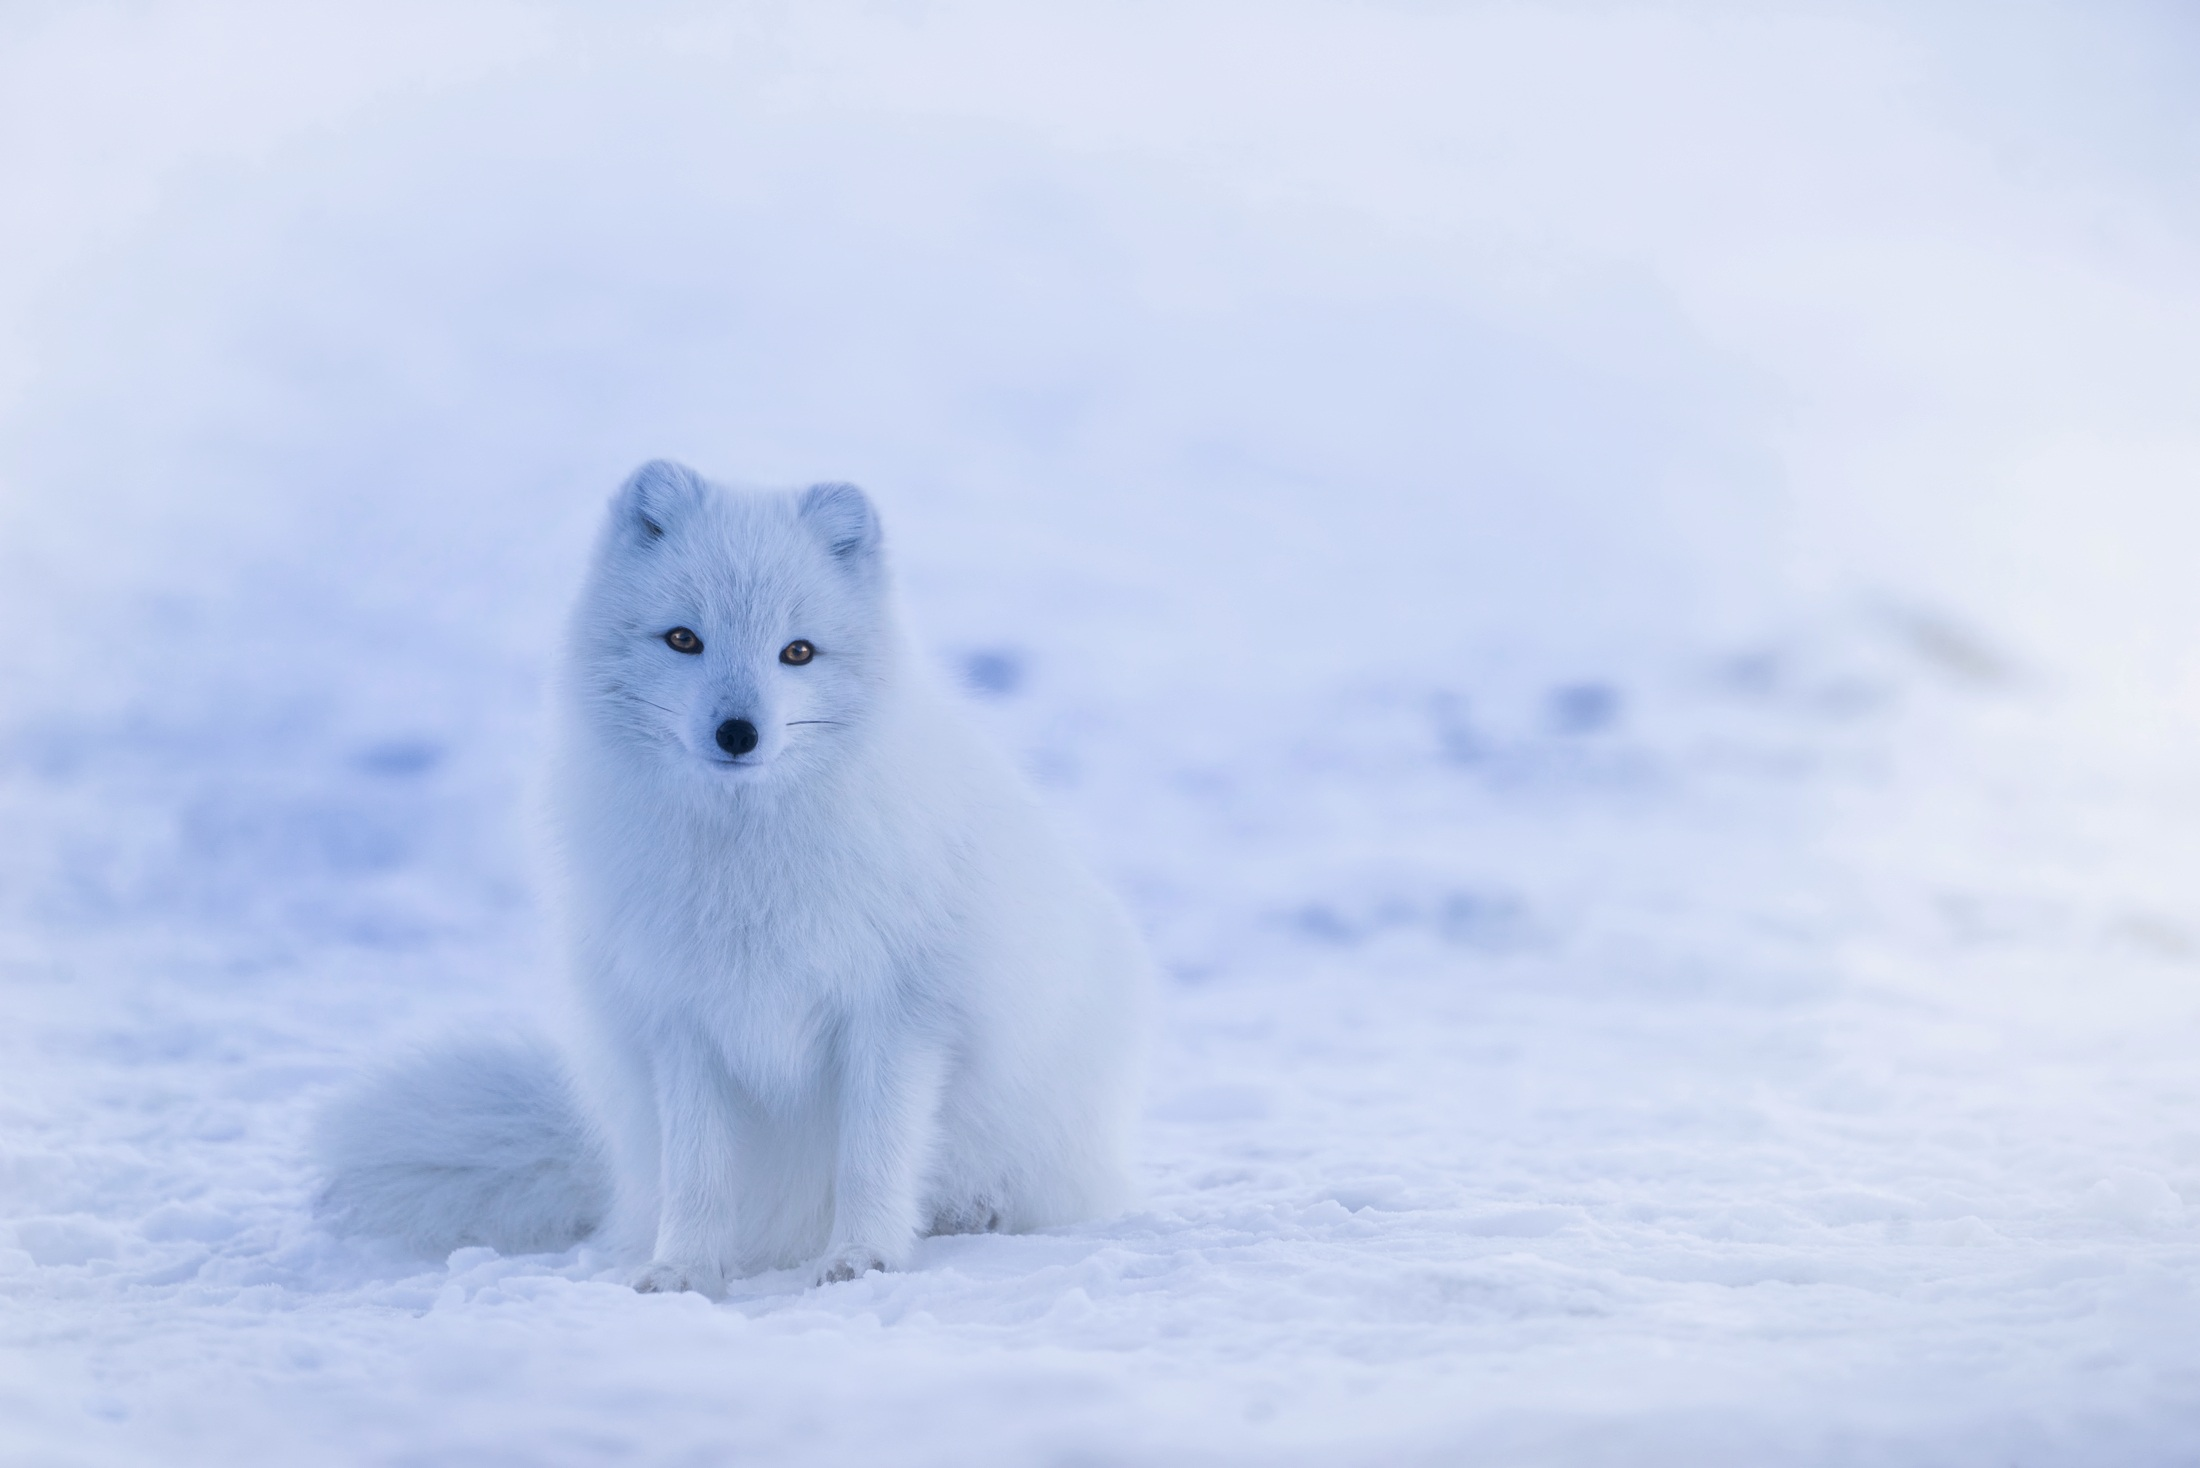
\includegraphics[scale = .5]{./image/test.jpg}
		\caption{图片标题}
		\label{fig:1-1}
	\end{figure}
	\subsection{多权重耦合神经网络的研究现状}
	近年来互联网的广泛使用引发了信息的爆炸式增长,个性化推荐系统作为解决“信息过载”问题的有效工具应运而生,通过算法帮助用户过滤信息,减少了用户需要处理的信息量。目前,个性化推荐系统已经广泛应用于搜索引擎、电子商务、社交娱乐等网络平台,在人们日常使用的过程中随处可见。然而,个性化推荐系统的广泛应用也带来了“信息窄化”、用户信息泄露等问题,个性化推荐系统对于用户信息搜寻成本的具体影响变得更为复杂。
	
	本文将用结构方程模型来分析信息搜寻成本的变化对个性化推荐系统的用户使用意愿的影响情况。
	
	基于研究得出的结论,本文从现实中存在的个性化推荐精度不足、信息窄化以及个人信息的侵害等方面的问题出发,提出了对于未来个性化推荐优化的展望。在算法方面,通过使用深度学习与知识图谱等前沿技术与算法提高个性化推荐的精确程度。在个人信息使用与信息窄化的问题上,平台可以增加相应调节选项,提高用户的自主选择性。其次,也可以通过提高推荐过程的可解释性来增强用户对推荐系统的信任度与满意度。另外,还需要政府部门完善个人信息保护的法律法规、社会舆论与公共部门发挥监督与监管作用,以及企业上下游齐发力,共同降低个人隐私泄露的风险。
	\subsection{预备知识}
		\subsubsection{符号介绍}
		%文献引用示例 请切换默认文献工具为biber
		文献引用\cite{孙鲁平2016网上个性化推荐研究述评与展望}
		\subsubsection{定理与引理}
		%公式引用示例
		\begin{equation}
			CR=\frac{\left (  \sum \lambda _{i}\right )^{2}}{\left [\left (  \sum \lambda _{i}\right )^{2}+\sum \theta   \right ]}
		\end{equation}
\subsection{本文的主要内容及结构}

\newpage
\section{多权重耦合神经网络的有限时间同步}
	\subsection{网络模型}
	近年来互联网的广泛使用引发了信息的爆炸式增长,个性化推荐系统作为解决“信息过载”问题的有效工具应运而生,通过算法帮助用户过滤信息,减少了用户需要处理的信息量。目前,个性化推荐系统已经广泛应用于搜索引擎、电子商务、社交娱乐等网络平台,在人们日常使用的过程中随处可见。然而,个性化推荐系统的广泛应用也带来了“信息窄化”、用户信息泄露等问题,个性化推荐系统对于用户信息搜寻成本的具体影响变得更为复杂。
	
	本文将用结构方程模型来分析信息搜寻成本的变化对个性化推荐系统的用户使用意愿的影响情况。
	
	基于研究得出的结论,本文从现实中存在的个性化推荐精度不足、信息窄化以及个人信息的侵害等方面的问题出发,提出了对于未来个性化推荐优化的展望。在算法方面,通过使用深度学习与知识图谱等前沿技术与算法提高个性化推荐的精确程度。在个人信息使用与信息窄化的问题上,平台可以增加相应调节选项,提高用户的自主选择性。其次,也可以通过提高推荐过程的可解释性来增强用户对推荐系统的信任度与满意度。另外,还需要政府部门完善个人信息保护的法律法规、社会舆论与公共部门发挥监督与监管作用,以及企业上下游齐发力,共同降低个人隐私泄露的风险。
	\subsection{有限时间的拓扑识别证明}
	\subsection{数值仿真}
	\subsection{本章小结}

\newpage
\section{多时滞耦合神经网络的有限时间同步}
	\subsection{网络模型}
	近年来互联网的广泛使用引发了信息的爆炸式增长,个性化推荐系统作为解决“信息过载”问题的有效工具应运而生,通过算法帮助用户过滤信息,减少了用户需要处理的信息量。目前,个性化推荐系统已经广泛应用于搜索引擎、电子商务、社交娱乐等网络平台,在人们日常使用的过程中随处可见。然而,个性化推荐系统的广泛应用也带来了“信息窄化”、用户信息泄露等问题,个性化推荐系统对于用户信息搜寻成本的具体影响变得更为复杂。
	
	本文将用结构方程模型来分析信息搜寻成本的变化对个性化推荐系统的用户使用意愿的影响情况。
	
	基于研究得出的结论,本文从现实中存在的个性化推荐精度不足、信息窄化以及个人信息的侵害等方面的问题出发,提出了对于未来个性化推荐优化的展望。在算法方面,通过使用深度学习与知识图谱等前沿技术与算法提高个性化推荐的精确程度。在个人信息使用与信息窄化的问题上,平台可以增加相应调节选项,提高用户的自主选择性。其次,也可以通过提高推荐过程的可解释性来增强用户对推荐系统的信任度与满意度。另外,还需要政府部门完善个人信息保护的法律法规、社会舆论与公共部门发挥监督与监管作用,以及企业上下游齐发力,共同降低个人隐私泄露的风险。
	\subsection{有限时间的拓扑识别证明}
	\subsection{数值仿真}
	\subsection{本章小结}

\newpage
\section{多权重耦合时滞神经网络的有限时间同步}
	\subsection{网络模型}
	\subsection{有限时间的拓扑识别证明}
	以显著性水平为0.05,结合上表数值即可判断本研究提出对的研究假设成立与否,结果如表\ref{tab:4-1}所示:
	
	表格采用三线表,如果超过一页显示范围,请以续表形式重启一页。
	\begin{table}[h]
		\centering
		\caption{表的标题}
		\label{tab:4-1}
		\begin{tabular}{@{}lll@{}}
			\toprule
			\bold{假设编号} & \textbf{研究假设}            & \bold{检验结果} \\ \midrule
			H1            & 时间成本降低对用户的个性化推荐使用意愿有正向影响 & 显著            \\
			H2            & 心理成本增加对用户的个性化推荐使用意愿有负向影响 & 显著            \\
			H3            & 金钱成本降低对用户的个性化推荐使用意愿有正向影响 & 显著            \\
			H4            & 风险成本增加对用户的个性化推荐使用意愿有负向影响 & 显著            \\ \bottomrule
		\end{tabular}
	\end{table}
	\subsection{数值仿真}
	\subsection{本章小结}

\newpage
\section{多时滞耦合时滞神经网络的有限时间同步}
	\subsection{网络模型}
	近年来互联网的广泛使用引发了信息的爆炸式增长,个性化推荐系统作为解决“信息过载”问题的有效工具应运而生,通过算法帮助用户过滤信息,减少了用户需要处理的信息量。目前,个性化推荐系统已经广泛应用于搜索引擎、电子商务、社交娱乐等网络平台,在人们日常使用的过程中随处可见。然而,个性化推荐系统的广泛应用也带来了“信息窄化”、用户信息泄露等问题,个性化推荐系统对于用户信息搜寻成本的具体影响变得更为复杂。
	
	本文将用结构方程模型来分析信息搜寻成本的变化对个性化推荐系统的用户使用意愿的影响情况。
	
	基于研究得出的结论,本文从现实中存在的个性化推荐精度不足、信息窄化以及个人信息的侵害等方面的问题出发,提出了对于未来个性化推荐优化的展望。在算法方面,通过使用深度学习与知识图谱等前沿技术与算法提高个性化推荐的精确程度。在个人信息使用与信息窄化的问题上,平台可以增加相应调节选项,提高用户的自主选择性。其次,也可以通过提高推荐过程的可解释性来增强用户对推荐系统的信任度与满意度。另外,还需要政府部门完善个人信息保护的法律法规、社会舆论与公共部门发挥监督与监管作用,以及企业上下游齐发力,共同降低个人隐私泄露的风险。
	\subsection{有限时间的拓扑识别证明}
	\subsection{数值仿真}
	\subsection{本章小结}

\newpage
\section{总结与展望}
	\subsection{总结}
	近年来互联网的广泛使用引发了信息的爆炸式增长,个性化推荐系统作为解决“信息过载”问题的有效工具应运而生,通过算法帮助用户过滤信息,减少了用户需要处理的信息量。目前,个性化推荐系统已经广泛应用于搜索引擎、电子商务、社交娱乐等网络平台,在人们日常使用的过程中随处可见。然而,个性化推荐系统的广泛应用也带来了“信息窄化”、用户信息泄露等问题,个性化推荐系统对于用户信息搜寻成本的具体影响变得更为复杂。
	
	本文将用结构方程模型来分析信息搜寻成本的变化对个性化推荐系统的用户使用意愿的影响情况。
	
	基于研究得出的结论,本文从现实中存在的个性化推荐精度不足、信息窄化以及个人信息的侵害等方面的问题出发,提出了对于未来个性化推荐优化的展望。在算法方面,通过使用深度学习与知识图谱等前沿技术与算法提高个性化推荐的精确程度。在个人信息使用与信息窄化的问题上,平台可以增加相应调节选项,提高用户的自主选择性。其次,也可以通过提高推荐过程的可解释性来增强用户对推荐系统的信任度与满意度。另外,还需要政府部门完善个人信息保护的法律法规、社会舆论与公共部门发挥监督与监管作用,以及企业上下游齐发力,共同降低个人隐私泄露的风险。
	\subsection{展望}

%v1.3add 修改 /begin
%参考文献
\newpage
%关闭页眉
\fancyhf{}
\renewcommand{\headrulewidth}{0pt}
\titleformat{\section}{\zihao{4}\raggedright\heiti\bold}{}{0em}{}
\cfoot{\footnotesize \thepage }
\printbibliography[heading=bibintoc,title={参考文献}]

%v1.3add 修改 /end

%附录
\newpage
\section*{\centerline{附\qquad 录}}
\addcontentsline{toc}{section}{附录}


%致谢
\newpage
\section*{\centerline{致\qquad 谢}}
\addcontentsline{toc}{section}{致谢}
我从进入大学到毕业整整四年。在这四年中,我过得浑浑愕额。四年前,我身高170cm,四年后,我身高还是170cm;四年前,我体重60kg,四年后,我体重还是60kg;四年前,我一无所有,四年后,我还是一无所有。四年前,我眼睛明亮、有神,四年后,摘掉眼镜,我已看不清自己有多少个手指了;四年前,我声音洪亮、清澈,四年后,已经是慢性咽喉炎,声音嘶哑;四年前,我踌躇满志、指点江山、激扬文字,四年后,我心如止水,只求温饱;当然,我也得到了一些东西。四年前,我还是个农民的儿子,四年后,我成为了一个博士;四年前,我只懂得砍柴、种田、割草、放牛,四年后,我已经成为了一个懂机械、金融、管理的复合型人才;但如果您问我这四年最大的长进是什么,我将告诉您:四年前,我四七,四年后,我二四七。

这四年中,我最渴望、最追求的是什么?是知识?不是。是美女?不是。而是钱。在我的脑海里,钱就是那种一块、一毛的硬币,我曾无数次翻天覆地的把它们找出来,目的就是去买一包方便面,吃一顿晚餐,而且找的时候不能太仔细了,太仔细了,下次就没有了。有时候,当我不知道下顿饭在哪里的时候,我想要是天上能掉下点钱就好了,我抬起头,只看到发黄的树叶正一片一片的落下来;我想要是能在地上捡点钱就好了,我低下头,只看见一些面包的包装纸以及一些插羊肉串的竹签。我从没见过天上掉过钱,也从没在地上捡过钱,所以我不相信有神的存在,因此我没有信仰。

衷心感谢我的恩师对我的淳淳教诲和悉心关怀,在我博士三年里,他给予了我生活上、学习上无微不至的关心。他也许是我四年大学生活里,唯一知道我名字的老师,也感谢他在承担100多个学生的指导任务下还能给我精心的指导。恩师对我的指导和影响之大,怎样言说都表达不尽,自己取得的点滴成绩无不凝聚着恩师的心血。恩师国际化的视野,前沿而精髓的学术造诣,严谨勤奋的治学风格,都让我永志不忘,深刻影响着我日后的工作和生活。

衷心感谢学院其他老师给予我的帮助。 衷心感谢各位同门师兄弟姐妹,感谢我们一起度过的苦难岁月。 衷心感谢我年迈的父母,我在这四年之中不忠不孝,没有让他们过上一天幸福的生活。他们还不停的支持我,关心我,鼓励我。经常问我“缺钱吗?”所以我相信亲情。我从不要他们的钱,我不想看到一百块钱,就想起几百个鸡蛋,几百担猪草,几千个红砖。 衷心感谢我的五个姐姐,是她们陪我度过快乐的童年。她们美丽纯真的少女时代唤起了我对异性的尊重与渴求。她们在我求学的四年中,不停的给我打电话,询问我的身体,生活,要我多吃点,给我寄钱,我也一直拒绝她们。这四年里,她们在广东的毛织厂、制衣厂过着非人的岁月。我不想看到那种用血、肉、生命、青春换来的东西。四年前,她们还是花一般的容颜,四年后,当她们出现在我的面前,我已经不相信她们就是我的姐姐了。

最后,我要感谢与我相茹以沫的女友×××,我们以总共不到600元的月收入,在上海和杭州这两个中国最发达的城市生活了5年。这5年里,我没有给她买过像样的礼物,而她却无数次在我青黄不接的日子里给我寄来她省吃俭用的钱,我才得以完成学业,所以我相信爱情。我无法明白她以275元的月收入,居然还可以救济我,或许她那纤细、苗条的身材就是最好的答案吧。

谨以此文献给千千万万的苦难中的学子们。[转自知乎]

\end{document}


























